
\lecture{Introduction to Bivariate Data}{introduction-to-bivariate-data}
\section{Introduction to Bivariate Data}

\title{Quantitative Data}
\subtitle{Methods to Assess Numerical Data}

%\author{Kelly Black}
%\institute{Clarkson University}
\date{5 February 2014}

\begin{frame}
  \titlepage
\end{frame}

\begin{frame}
  \frametitle{Outline}
  \tableofcontents[hideothersubsections,sectionstyle=show/hide]
\end{frame}


\subsection{Clicker Quiz}


\iftoggle{clicker}{%
  \begin{frame}
    \frametitle{Clicker Quiz}

    A normally distributed random variable has a mean of 1.2. The
    probability that it is less than 0.8 is 0.25. What is the standard
    deviation?
    
    \vfill

    \begin{tabular}{l@{\hspace{3em}}l@{\hspace{3em}}l@{\hspace{3em}}l}
      A: -0.67 & B: -0.40  & C: 0.60 & D: 0.67
    \end{tabular}

    \vfill

  \end{frame}
}


\subsection{Quantitative Data}

\begin{frame}{Quantitative Data}
  
  \begin{definition}{Discrete Data}

    A discrete random variable produces a countable number of
    values. The values are one of a fixed set of values. 

    \textit{{\color{red}Here the random variables are numbers.}}
    
  \end{definition}

  \begin{definition}{Continuous Data}

    The numbers produced come from a continuous range of values.
    
  \end{definition}

\end{frame}

\begin{frame}{Discrete Data Examples}

  \begin{itemize}
  \item Count the number of people who arrive in a line during a given
    time period.

  \item We report the number of bottles of a brand of soft drink that
    are sold in a given time period.

  \item We report the number of defects found in a mirror randomly
    chosen from a factory floor.

  \end{itemize}
  
\end{frame}


\begin{frame}{Quantitative Data}
  
  \begin{definition}[Univariate Data]

    Each observation consists of a measurement, and there are no
    explicit relationships between them.

    \textit{{\color{red}All of the examples on the previous slide
        represent univariate data.}}
    
  \end{definition}

  \begin{definition}[Bivariate Data]

    Each observation consists of a pair of measurements.
    
  \end{definition}

  \begin{definition}[Multivariate Data]

    Each observation consists of more than two measurements. There is
    more than two measurements per group.
    
  \end{definition}


\end{frame}



\subsection{Bivariate Data}

\begin{frame}
  \frametitle{Bivariate Data}

  \begin{eqnarray*}
    \begin{array}{l|l}
      x      & y \\ \hline 
      x_1    & y_1 \\
      x_2    & y_2 \\
      \vdots & \vdots \\
      x_n    & y_n
    \end{array}
  \end{eqnarray*}
\end{frame}



\iftoggle{clicker}{%
  \begin{frame}
    \frametitle{Clicker Quiz}

    An experiment is run in which an intersection is observed over
    twenty different two hour periods, and the number of people who do
    not stop at a stop sign is observed.

    What kind of data is this?

    \vfill

    \begin{tabular}{l@{\hspace{3em}}l@{\hspace{3em}}l@{\hspace{3em}}l}
      A: univariate, discrete & B: univariate, continuous  \\
      C: bivariate, discrete  & D: bivariate, continuous
    \end{tabular}

    \vfill



  \end{frame}
}

\subsection{Discrete Quantitative Data}

\begin{frame}
  \frametitle{Discrete Quantitative Data}

  \begin{eqnarray*}
    5,~5,~3,~5,~4,~3,~4,~1,~6,~3,~2,~1
  \end{eqnarray*}

  This is no different from what we did with qualitative data in our
  last session. Just count the number of occurrences and work with
  frequencies.


  \only<2->%
  {
    \begin{tabular}{l|l}
      Number  & Frequency \\ \hline
      1 & 2 \\
      2 & 1 \\
      3 & 3 \\
      4 & 2 \\
      5 & 3 \\
      6 & 1 
    \end{tabular}
  }

  \only<3->%
  {
    \textit{relative frequency, blah blah blah}
  }

\end{frame}

\subsection{Continuous Data}

\begin{frame}
  \frametitle{Continuous Data}

  \begin{itemize}
  \item Every day I measure the amount of precipitation over the
    previous 24 hours.

  \item I observe the price of a particular stock at the end of each day.
    \uncover<2->{\textit{\color{red}Well... technically this is discrete, but we
        pretend it is continuous.}}

  \item I measure the blood alcohol levels for people who have been
    pulled over each night in Potsdam, NY.
  \end{itemize}
\end{frame}

\subsection{Graphical Techniques}

\begin{frame}{Graphical Techniques}

  \begin{itemize}
  \item Bar Plots
  \item Dot Plots
  \item Stem-Leaf Charts
  \item histograms
  \end{itemize}
  
\end{frame}


\begin{frame}{Bar Plots}

  \begin{eqnarray*}
    5,~5,~3,~5,~4,~3,~4,~1,~6,~3,~2,~1
  \end{eqnarray*}


  \begin{columns}
    \column{.25\textwidth}


    \begin{tabular}{l|l}
      Number  & Frequency \\ \hline
      1 & 2 \\
      2 & 1 \\
      3 & 3 \\
      4 & 2 \\
      5 & 3 \\
      6 & 1 
    \end{tabular}

    \column{.75\textwidth}

    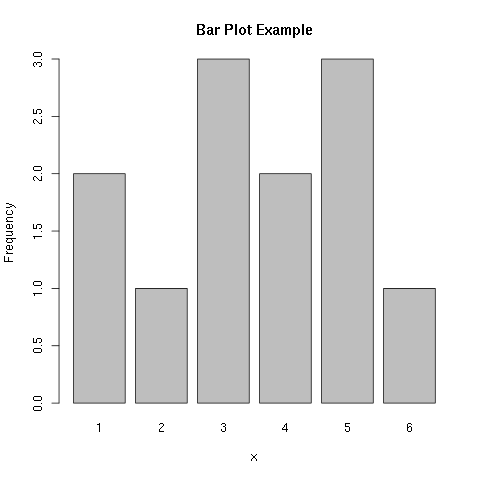
\includegraphics[width=7cm]{img/barplotExample}


  \end{columns}
  
  
\end{frame}


\begin{frame}{Dot Charts}

  \begin{eqnarray*}
    5,~5,~3,~5,~4,~3,~4,~1,~6,~3,~2,~1
  \end{eqnarray*}


  \begin{columns}
    \column{.25\textwidth}


    \begin{tabular}{l|l}
      Number  & Frequency \\ \hline
      1 & 2 \\
      2 & 1 \\
      3 & 3 \\
      4 & 2 \\
      5 & 3 \\
      6 & 1 
    \end{tabular}

    \column{.75\textwidth}

    \only<1>{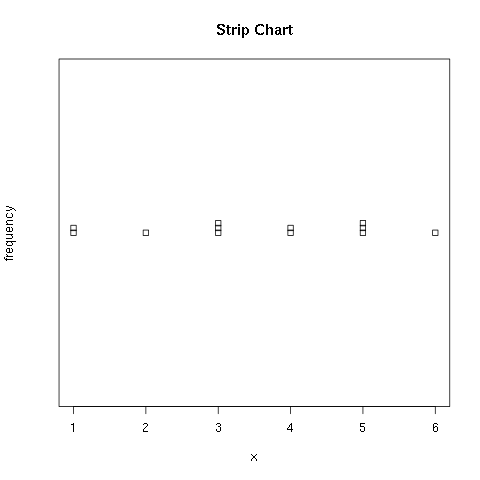
\includegraphics[width=7cm]{img/stripChart}}
    \only<2>{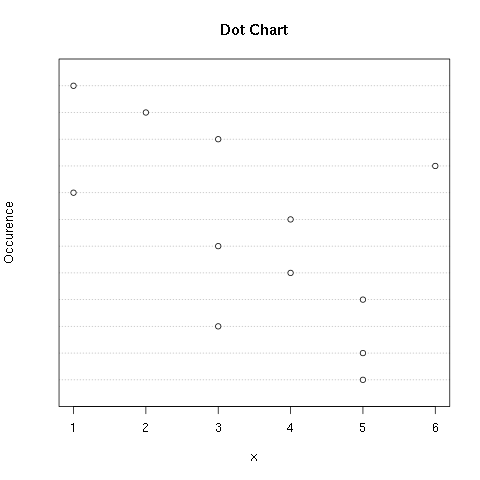
\includegraphics[width=7cm]{img/dotChart}}


  \end{columns}
  
  
\end{frame}


\begin{frame}{Stem-Leaf Plot}

  We can divide a number between its ``stem'' and ``leaf.''

  For example:
  \only<1>%
  {
    \begin{eqnarray*}
      17
    \end{eqnarray*}
  }
  \only<2>%
  {
    \begin{eqnarray*}
      \underbrace{\color{red}1}_{\mathrm{stem}}\underbrace{\color{blue}7}_{\mathrm{leaf}}
    \end{eqnarray*}
  }

  \only<3>%
  {
    Given a group of numbers we can organize the numbers with the same
    stem in the same rows. Then list each leaf in ascending order. The
    result is a ``stem-leaf plot.''
  }
  
  
\end{frame}

\begin{frame}{Example}

  \only<1>%
  {
    \begin{eqnarray*}
      47,~44,~29,~27,~29,~36,~24,~21,~36,~34
    \end{eqnarray*}
  }
  \only<2>%
  {
    Identify the stems:
    \begin{eqnarray*}
      {\color{red}4}7,~{\color{red}4}4,~{\color{red}2}9,~{\color{red}2}7,
      ~{\color{red}2}9,~{\color{red}3}6,~{\color{red}2}4,~{\color{red}2}1,
      ~{\color{red}3}6,~{\color{red}3}4
    \end{eqnarray*}
  }\
  \only<3->%
  {
    Identify the leaves:
    \begin{eqnarray*}
      {\color{red}4}{\color{blue}7},~{\color{red}4}{\color{blue}4},
      ~{\color{red}2}{\color{blue}9},~{\color{red}2}{\color{blue}7},
      ~{\color{red}2}{\color{blue}9},~{\color{red}3}{\color{blue}6},
      ~{\color{red}2}{\color{blue}4},~{\color{red}2}{\color{blue}1},
      ~{\color{red}3}{\color{blue}6},~{\color{red}3}{\color{blue}4}
    \end{eqnarray*}
  }

  \only<4>%
  {
    Write out the unique stems in order: \\
    \begin{tabular}{l@{\hspace{1em}}|@{\hspace{1em}}l}
      {\color{red}2} & \\
      {\color{red}3} & \\
      {\color{red}4} & 
    \end{tabular}
  }

  \only<5>%
  {
    Write out every leaf in ascending order: \\
    \begin{tabular}{l@{\hspace{1em}}|@{\hspace{1em}}l}
      {\color{red}2} & {\color{blue}14799}\\
      {\color{red}3} & {\color{blue}466}\\
      {\color{red}4} & {\color{blue}47}
    \end{tabular}
  }

  
\end{frame}

\begin{frame}{Histograms}

  This is a generalization of the stem-leaf plot. Instead of dividing
  things in groups by the ``tens'' we instead use an arbitrary range
  of values. We calculate how many data points fall into the
  pre-determined ranges and then make a bar plot of the frequencies.
  
\end{frame}

\begin{frame}{Example}

  \begin{eqnarray*}
    2.7,~3.6,~3.8,~2.7,~2.7,~3.3,~3.3,~3.6,~3.0,~3.2
  \end{eqnarray*}


  \begin{columns}
    \column{.25\textwidth}

    \only<2>%
    {
      We (arbitrarily) break things up into a range of values: \\
      \begin{tabular}{l|l}
        2.6-2.8 \\
        2.8-3.0 \\
        3.0-3.2 \\
        3.2-3.4 \\
        3.4-3.6 \\
        3.6-3.8
      \end{tabular}
    }

    \only<3->%
    {
      We (arbitrarily) break things up into a range of values: \\
      \begin{tabular}{l|l}
        2.6-2.8 & III\\
        2.8-3.0 & I \\
        3.0-3.2 & I \\
        3.2-3.4 & II \\
        3.4-3.6 & II \\
        3.6-3.8 & I
      \end{tabular}
    }
    
    \column{.75\textwidth}

    \only<4>{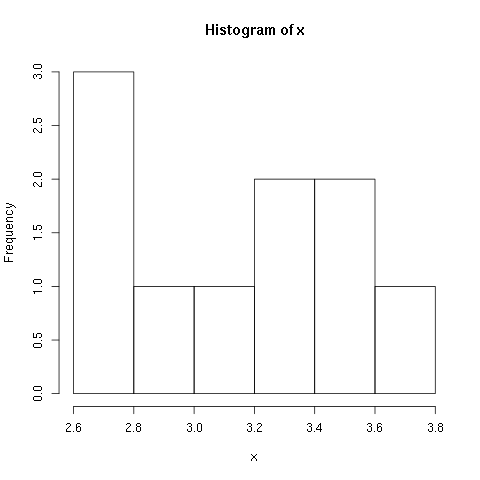
\includegraphics[width=6cm]{img/histogramExample}}

  \end{columns}

  
\end{frame}

\begin{frame}{Histograms}

  \begin{itemize}
  \item Overall shape 
  \item Skew
  \item Center (balance point, middle of area)
  \item Spread
  \end{itemize}
  
\end{frame}

% LocalWords:  Clarkson pausesection hideallsubsections Bivariate
